\documentclass{article}
\usepackage{amsmath, amssymb}
\usepackage{pgfplots}
\usepackage{tikz}
\usepackage{booktabs}
\usepackage{xcolor}
\usepackage{tcolorbox}


% page 541 has a good amout of information

\begin{document}


\title{Chapter 19}
\author{}
\date{}

\maketitle



\section*{What is the first law of Thermodynamics?}

To sum it up the first law of Thermodynamics is energy transferring into/out of the system as work or heat



\begin{equation}
    \Delta E_{\text{th}} = W + Q
\end{equation}

where:
\begin{itemize}
    \item $\Delta E_{\text{th}}$ = Change in thermal energy (J)
    \item $W$ = Work done on the system (J)
    \item $Q$ = Heat added to the system (J)
\end{itemize}


\section*{19.2 Work in Ideal-Gas Processes}

\begin{equation}
    W = - \int_{V_i}^{V_f} P \, dV
\end{equation}

\section*{Isochoric Process}

\begin{equation}
    W = 0
\end{equation}
Isochoric process is a process in which the volume of the system is constant and the work done is zero.


\section*{Isobaric Process}

    \begin{equation}
        W = - P \Delta V
    \end{equation}
    Isobaric process is a process in which the pressure of the system is constant and the work done is $-P \Delta V$.
    where:
    
    
    \begin{itemize}
        \item $W$ = Work done on the system (J)
        \item $P$ = Pressure of the gas (Pa)
        \item $\Delta V$ = Change in volume of the gas (m$^3$)
    \end{itemize}

\section*{isothermal Process}

\begin{equation}
    W = - nRT \ln \left( \frac{V_f}{V_i} \right) = - p_i V_i \ln \left( \frac{V_f}{V_i} \right) = - p_f V_f \ln \left( \frac{V_f}{V_i} \right)
\end{equation}

where:
\begin{itemize}
    \item $n$ = Number of moles of the gas (mol)
    \item $R$ = Ideal gas constant (8.31 J/mol $\cdot$ K)
    \item $T$ = Temperature of the gas (K)
    \item $V_i$ = Initial volume of the gas (m$^3$)
    \item $V_f$ = Final volume of the gas (m$^3$)
    \item $p_i$ = Initial pressure of the gas (Pa)
    \item $p_f$ = Final pressure of the gas (Pa)
\end{itemize}


\vspace{1cm}

\begin{equation}
    \Delta E_{\text{th}} = 0
\end{equation}


\section*{Adiabatic Process}
Def: An adiabatic process is a process in which no heat is added to or removed from the system.

\section*{Heat}

to be continue

\section*{19.3.2 Units of Heat}

\begin{equation}
    1 \text{ cal} = 4.186 \text{ J}
\end{equation}


\vspace{2cm}




\begin{table}[h]
    \centering
    \section*{19.5.1 Specific Heat and molar specifc heats of solids and liquids}
    \begin{tabular}{lcc}
        \toprule
        \textbf{Substance} & \textbf{$c$ (J/kg K)} & \textbf{$C$ (J/mol K)} \\
        \midrule
        \multicolumn{3}{l}{\textbf{Solids}} \\
        Aluminum  & 900  & 24.3 \\
        Copper    & 385  & 24.4 \\
        Iron      & 449  & 25.1 \\
        Gold      & 129  & 25.4 \\
        Lead      & 128  & 26.5 \\
        Ice       & 2090 & 37.6 \\
        \midrule
        \multicolumn{3}{l}{\textbf{Liquids}} \\
        Ethyl alcohol & 2400 & 110.4 \\
        Mercury       & 140  & 28.1 \\
        Water         & 4190 & 75.4 \\
        \bottomrule
    \end{tabular}
\end{table}

\vspace{2cm}


\begin{equation}
    Q = mc \Delta T
\end{equation}

where:
\begin{itemize}
    \item $Q$ = Heat added to the system (J)
    \item $m$ = Mass of the substance (kg)
    \item $c$ = Specific heat of the substance (J/kg K)
    \item $\Delta T$ = Change in temperature of the substance (K)
\end{itemize}

\vspace{2cm}

\begin{equation}
    Q = nC \Delta T
\end{equation}

where:
\begin{itemize}
    \item $Q$ = Heat added to the system (J)
    \item $n$ = Number of moles of the substance (mol)
    \item $C$ = Molar specific heat of the substance (J/mol K)
    \item $\Delta T$ = Change in temperature of the substance (K)
\end{itemize}


\section*{19.5.2 Phase Changes and Heat of Transformation}

Phase changes are changes in the state of a substance, such as from solid to liquid or from liquid to gas.

\begin{tcolorbox}
    \begin{equation}
        Q = mL \quad \text{(phase change)}
    \end{equation}
\end{tcolorbox}

\quad

\begin{tcolorbox}
    \begin{equation}
        Q =
        \begin{cases} 
          \pm M L_f & \text{melt/freeze} \\
          \pm M L_v & \text{boil/condense}
        \end{cases}
    \end{equation}
\end{tcolorbox}

\quad


\begin{table}[h]
    \centering
    \caption{Melting/boiling temperatures and heats of transformation}
    \begin{tabular}{l c c c c}
        \toprule
        \textbf{Substance} & $T_m$ (°C) & $L_f$ (J/kg) & $T_b$ (°C) & $L_v$ (J/kg) \\
        \midrule
        Nitrogen ($N_2$) & $-210$ & $0.26 \times 10^5$ & $-196$ & $1.99 \times 10^5$ \\
        Ethyl alcohol & $-114$ & $1.09 \times 10^5$ & $78$ & $8.79 \times 10^5$ \\
        Mercury & $-39$ & $0.11 \times 10^5$ & $357$ & $2.96 \times 10^5$ \\
        Water & $0$ & $3.33 \times 10^5$ & $100$ & $22.6 \times 10^5$ \\
        Lead & $328$ & $0.25 \times 10^5$ & $1750$ & $8.58 \times 10^5$ \\
        \bottomrule
    \end{tabular}
\end{table}


\section*{19.6 Caloriemtery}

calorimetery: 


\section*{19.7 The Specific Heats of Gases}

\begin{equation}
    Q = nC_V \Delta T \quad \text{(temperature change at constand Volume)}
\end{equation}

\begin{equation}
    Q = nC_P \Delta T \quad \text{(temperature change at constant Pressure)}
\end{equation}

where:
\begin{itemize}
    \item $Q$ = Heat added to the system (J)
    \item $n$ = Number of moles of the gas (mol)
    \item $C_V$ = Molar specific heat of the gas at constant volume (J/mol K)
    \item $C_P$ = Molar specific heat of the gas at constant pressure (J/mol K)
    \item $\Delta T$ = Change in temperature of the gas (K)
\end{itemize}

\begin{table}[h]
    \centering
    \renewcommand{\arraystretch}{1.3}
    \setlength{\tabcolsep}{10pt}
    \begin{tabular}{lccc}
        \toprule
        \textbf{Gas} & $C_P$ & $C_V$ & $C_P - C_V$ \\
        \midrule
        \multicolumn{4}{l}{\textbf{Monatomic Gases}} \\
        He & 20.8 & 12.5 & 8.3 \\
        Ne & 20.8 & 12.5 & 8.3 \\
        Ar & 20.8 & 12.5 & 8.3 \\
        \midrule
        \multicolumn{4}{l}{\textbf{Diatomic Gases}} \\
        H$_2$ & 28.7 & 20.4 & 8.3 \\
        N$_2$ & 29.1 & 20.8 & 8.3 \\
        O$_2$ & 29.2 & 20.9 & 8.3 \\
        \bottomrule
    \end{tabular}
    \caption{Molar specific heats of gases (J/mol K) at $T = 0^\circ C$}
    \label{tab:specific_heats}
\end{table}


\quad

\begin{tcolorbox}[colback=yellow!15, colframe=black, sharp corners, boxrule=1pt, width=\textwidth]
    \begin{equation} 
        C_P - C_V = R
        \quad
        \text{or}
        \quad
        C_P = C_V + R
    \end{equation}
\end{tcolorbox}

\begin{equation}
    \Delta E_\text{th} = nC_V \Delta T \quad \text{(any ideal-gas process)}
\end{equation}


\section*{19.7.3 Adiabatic Processes}

\noindent \textbf{FIGURE 19.19} \quad \textbf{The relationship of three important processes to the first law of thermodynamics.}

\vspace{0.5cm}

\begin{center}
    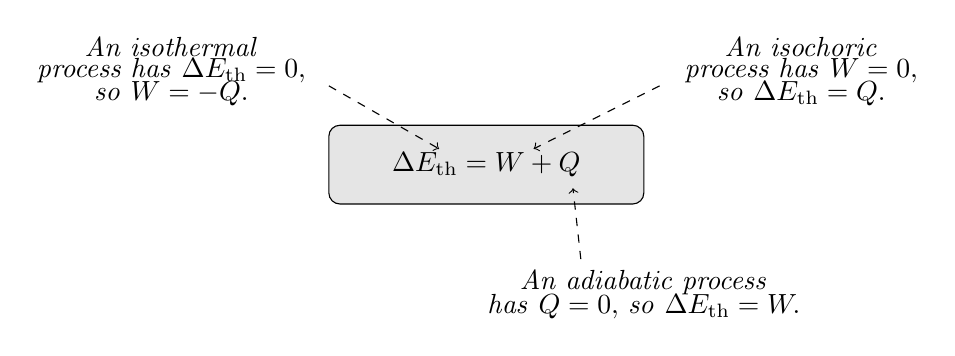
\begin{tikzpicture}
        % Main equation box
        \node at (0,0) [draw, fill=gray!20, rounded corners, minimum width=4cm, minimum height=1cm] 
            {$\Delta E_{\text{th}} = W + Q$};
        
        % Isothermal process
        \node at (-4, 1.5) {\textit{An isothermal}};

        \node at (-4, 1.2) {\textit{process has} $\Delta E_{\text{th}} = 0,$};
        \node at (-4, 0.9) {\textit{so} $W = -Q.$};
        \draw[->, dashed] (-2, 1) -- (-0.6, 0.2);
        
        % Isochoric process
        \node at (4, 1.5) {\textit{An isochoric}};
        \node at (4, 1.2) {\textit{process has} $W = 0,$};
        \node at (4, 0.9) {\textit{so} $\Delta E_{\text{th}} = Q.$};
        \draw[->, dashed] (2.2, 1) -- (0.6, 0.2);
        
        % Adiabatic process
        \node at (2, -1.5) {\textit{An adiabatic process}};
        \node at (2, -1.8) {\textit{has} $Q = 0,$ \textit{so} $\Delta E_{\text{th}} = W.$};
        \draw[->, dashed] (1.2, -1.2) -- (1.1, -0.3);
    \end{tikzpicture}
\end{center}

\quad

\begin{tcolorbox}[colback=yellow!15, colframe=black, sharp corners, boxrule=1pt, width=\textwidth]
    \begin{equation}
       W = nC_V \Delta T \quad \text{(adiabatic process)}
    \end{equation}
\end{tcolorbox}

\subsection{Specific Hear Ratio $\gamma$}

\begin{tcolorbox}[colback = red!15, colframe=black, sharp corners, boxrule=1pt, width=\textwidth]
    \begin{equation}
        \gamma = \frac{C_P}{C_V}
    \end{equation}
\end{tcolorbox}
\quad
An adiabatic process is one in which

\begin{tcolorbox}
    \begin{equation}
        pV^\gamma = \text{constant} \quad \textsl{or} \quad p_i V_i^\gamma = p_f V_f^\gamma
    \end{equation}
\end{tcolorbox}


%Start of the addtion notes page
\section*{Addtional Notes}
when you want to find M (molar mass) you can use the following formula:
\begin{equation}
    M = \frac{m}{n}
\end{equation}

Find the number from the periodic table and divide it by the number of moles of the gas to find the molar mass of the gas.

where:
\begin{itemize}
    \item $M$ = Molar mass (kg/mol)
    \item $m$ = Mass of the gas (kg) usally given in grams
    \item $n$ = Number of moles of the gas (mol)
\end{itemize}


\section*{Finding the number of moles of the gas}
\begin{equation}
    n = \frac{\text{mass of the gas}}{\text{molar mass of the gas}}
\end{equation}

\section*{Celsius scale to Kelvin scale conversion}
\begin{tcolorbox}
    \begin{equation}
        T_K = T_C + 273
    \end{equation}
\end{tcolorbox}

\section*{Find mass with given Volume}
Usally these probelms give you Volume and wonder how do we get mass.

We have to take a look at the period table and find density.

After that we can now use the following formula to find mass:

\begin{tcolorbox}
    \begin{equation}
        m = \rho V
    \end{equation}
\end{tcolorbox}


\end{document}